\documentclass[Analysis-3]{subfiles}
\usepackage{style}

\begin{document}
\chapter*{Lecture 23} %Set chapter name
\addcontentsline{toc}{chapter}{Lecture 23} %Set chapter title
\setcounter{chapter}{23} %Set chapter counter
\setcounter{section}{0}
We will begin this lecture with few examples.
\begin{Eg}{Path Of a Projectile}
    . \begin{align*}
        \gamma(t)&=(\alpha t,\beta t-16t^2)\\
        \implies \gamma'(t) &= (\alpha ,\beta -32t)\\
        \text{path length} &= \int||\gamma'(t)|| dt \\
        &= \int \sqrt{\alpha^2 +(\beta-32t)^2} dt
      \end{align*}
\end{Eg}

\begin{Eg}{Perimeter of a Circle}
 . Parametrization of a circle of radius $r$ is given by $\gamma(t) = (r\cos(t),r\sin(t)), t \in [0,2\pi)$.
 \begin{align*}
    \gamma'(t) &= (-r\sin(t),r\cos(t)) \\
    \ell (\gamma) &= \int_{0}^{2\pi} ||\gamma'(t)|| dt \\
    &= \int_{0}^{2\pi} r dt \\
    &= 2\pi r 
 \end{align*}
\end{Eg}

\begin{Eg}{Arc Length of graph of functions}
    .Let,$f : [a,b]\to \mathbb{R}$ be a $C^1$ function. Consider $\gamma(t)=(t,f(t))$. It is a smooth curve.
    \begin{align*}
        \gamma'(t) &= (1,f'(t)) \\
     \ell (\gamma) &= \int_{a}^{b} ||\gamma'(t)|| dt \\
     &= \int_{a}^{b} \sqrt{1 + f'(t)^2} dt
    \end{align*}
\end{Eg}

\section{Line Integrals}
To integrate a function over a curve we use \textbf{Line integral}.The function we should integrate maybe a \textbf{Scaler Field} or a \textbf{Vector Field}.(A quick example of a Vector Field: $f : \mathcal{O}_n \to \R$ be a differentiable function, then $\nabla f$ is a vector field.)

\textbf{Question :} Given a scaler field $f : \mathcal{O}_n \to \R$ and $\gamma \equiv c$ be a curve, we want to define $\int_c f$ . But exactly how we can do this? 

\textbf{Answer :} $c$ is a curve so it is bounded suset of $\R^n$. How about thinking of \textbf{Riemann Integration} ? for $n \ge 2$, $c$ is \textbf{content zero} in $\R^n$. This does not make nay sense ! The right way is as following .

\vspace*{0.5cm}

Let, $\gamma :[a,b]\to \R^n$ be a \textbf{Smooth curve}(Or Pieecewise Smooth) and $c:= \text{ran}(\gamma)$( on other words path of $\gamma$). Let, $f \in \mathscr{B}(c)$. Given $\mathcal{P} \in \mathscr{P}[a,b]$, $\mathcal{P} : a = t_0<t_1<\cdots <t_m = b$.
  
\vspace{0.2cm}

\begin{wrapfigure}{r}{0.5\textwidth}
    \centering
    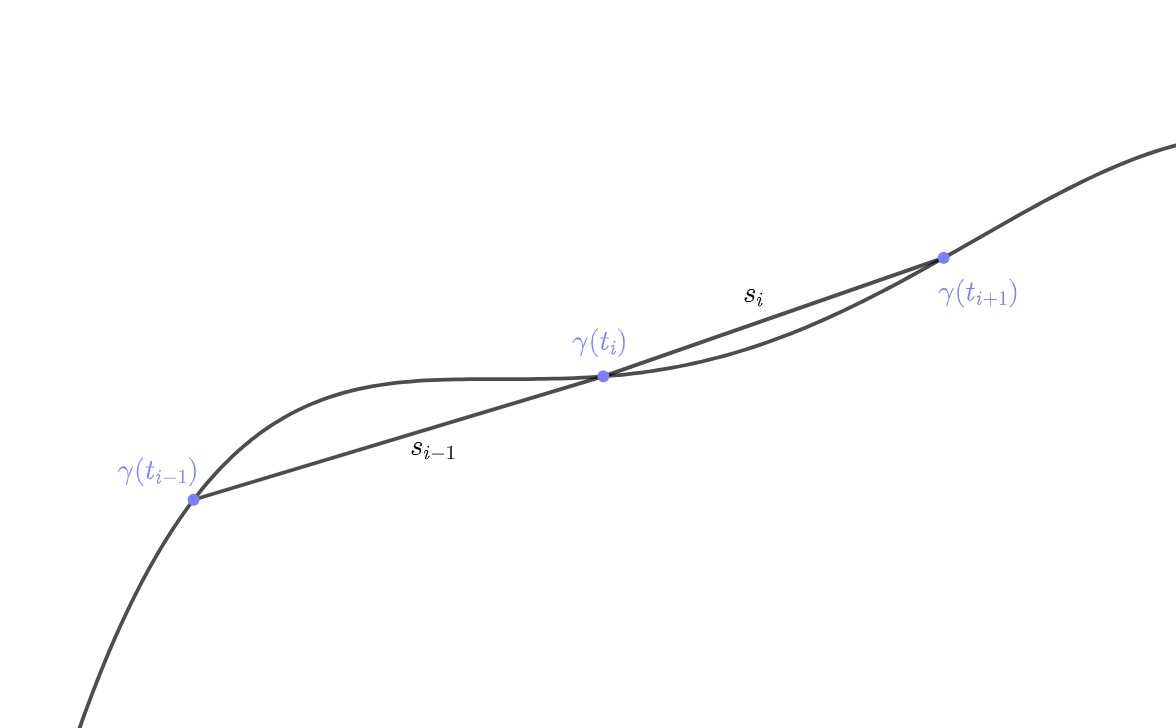
\includegraphics[width=.98\linewidth]{figures/lec-23.1.png}
    \caption{Curve $c$}
\end{wrapfigure}
Let, $I_i = [t_{i-1},t_i]$ be the subintervals and $c_i = \gamma(I_i)$. 
Since,$\gamma$ is smooth there is nice correspondance between $I_i$ and $c_i$. Also denote $s_i$ by $||\gamma(t_i) - \gamma(t_i)||$.As previous, define $m_i = \inf_{c_i}f$ and $M_i = \sup_{c_i}f$.
\begin{align*}
    U(f,\mathcal{P}) &= \sum_{i=1}^{m}M_i.s_i \\
    L(f,\mathcal{P}) &= \sum_{i=1}^{m}M_i.s_i 
\end{align*}
The above expressions are same as upper and \vspace{0.05cm} 

lower Riemann sum respectively. This opens up 

"\textcolor{violet}{The Pandora's box !} ".
\vspace{0.3cm}

$\bullet$ We can now use all the theory we used for the standared Riemann Integrals.We say $f$ is line integrable over $\gamma$ if, 
\[\inf_{\mathcal{P} \in \mathscr{P}[a,b]} U(f,\mathcal{P}) = \sup_{\mathcal{P} \in \mathscr{P}[a,b]} L(f,\mathcal{P})\]

More over we will write the common value of the above equality as $\int_c f$ and call this "The Line Integral over curve $c$".



\end{document}